\documentclass[a4paper]{article}
\usepackage{amsmath}
\usepackage{amsfonts}
\usepackage{amsthm}
\usepackage{amssymb}
\usepackage[english]{babel}
\usepackage{float}
\usepackage{graphicx}
\usepackage{hyperref}
\usepackage[utf8]{inputenc}
\usepackage{listings}
\usepackage{xcolor}
%% \usepackage{subfigure}
\usepackage{graphicx}
\usepackage{subcaption}
\usepackage{stmaryrd}

\usepackage{a4wide}
\usepackage{url}
%% \usepackage[left=2cm,top=2cm,bottom=1.5cm,right=2cm]{geometry}

\lstset{
  frame=tb,
  language=Python,
  aboveskip=3mm,
  belowskip=3mm,
  showstringspaces=false,
  formfeed=newpage,
  tabsize=4,
  comment=[l]{\#},
  breaklines=true,
  morekeywords={models, lambda, forms}
}

\newcommand{\prob}[1]{\mathbb{P}\left(#1\right)}
\newcommand{\expect}[1]{\mathbb{E}\left(#1\right)}
\newcommand{\avg}[1]{\sum_{i=1}^{#1}X_i}
\newcommand*{\QEDA}{\hfill\ensuremath{\blacksquare}}%

\title{\vspace{-5cm} Numerical Optimization \\ Handin 1 - Peer Review}
\author{Dmitry Serykh (qwl888)}

\begin{document}
\maketitle
\section{Introduction}
\label{intro}
I am reviewing the report by Michael Emil Rosenstrøm (kfg364).

\section{Review}
\label{sec:review}
\subsection{General Structure}
The report is structured as a sequence of isolated sections. An alternative
format could be chosen, where the whole report would be logically connected and
the reader could follow the overarching line of thought.

\subsection{Plots}
The plots for all five functions are provided. Furthermore, two types of plots
for each are included: a surface plot and a curve plot. The former is useful for
getting an overview of the shape of the functions, but finer details could be
obfuscated. The latter can be used to get the finer details, especially around
the saddle points of the functions. However, the color-bar on the curve plot is hard to read
because the boxes are not filled with colors. That could be easily mitigated by
choosing a different color-bar style.

The curve plot could further be supplied
by a ``temerature-plot'' using \texttt{imshow}, that way even more finer details
of the function could be captured. Furthermore, the contour plot could be made
easier to read by making the surface transparent.

The biggest problem with this report is the lack of argumentation for the
correctness of the given plots. Most of the parts from the theoretical parts
should have been included in the discussion.

\subsection{Theoretical Part}
The proofs for the Hessian matrix and minimizers of Rosenbrock and Ellipsoid
functions are provided and easy to follow. However, the argument for the
gradient correctness is lacking and could have been argued for using the Taylor
Theorem. The gradient and Hessians for all functions are provided.

The proof for correctness of the re-formulation of the $\log{1 + \exp{x}}$ is
provided. However, the actual argument for why the alternative formulation is
better is missing.


%% \begin{figure}
%%   \centering
%%     \centering
%%     \includegraphics[scale=1]{code/plt_p21}
%%   \caption{Plot for the generated dataset}
%%   \label{plt_p21}
%% \end{figure}

%% \begin{lstlisting}[caption="Calculation of g"]
%% def calc_g(Xs, y, w):
%%     N = np.shape(Xs)[0]
%%     # use matrix X of xs instead of for-loop = much faster
%%     X = np.c_[Xs, np.ones(N)]
%%     num = y.T * X
%%     denum = 1 + np.exp(y * (w @ X.T))
%%     M = num.T/denum
%%     # return mean of each row
%%     return (-1 * np.mean(M, axis=1))
%% \end{lstlisting}


%% \begin{figure}
%%   \centering
%%   \begin{subfigure}[b]{\textwidth}
%%     \centering
%%     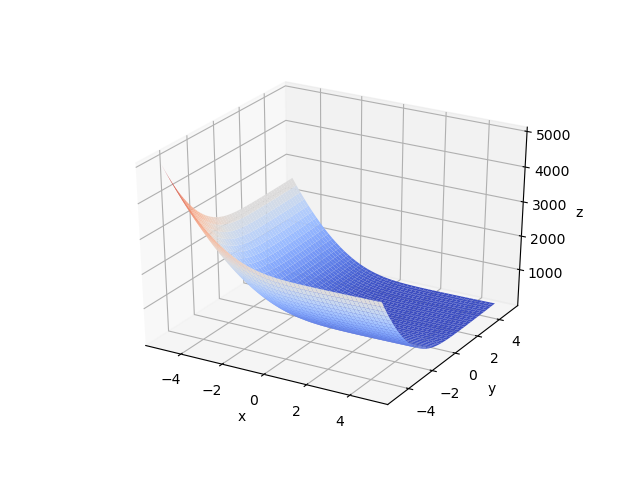
\includegraphics[scale=0.8]{handin/plt51}
%%     \caption{Classification of the training set}
%%   \end{subfigure}
%%   \begin{subfigure}[b]{\textwidth}
%%     \centering
%%     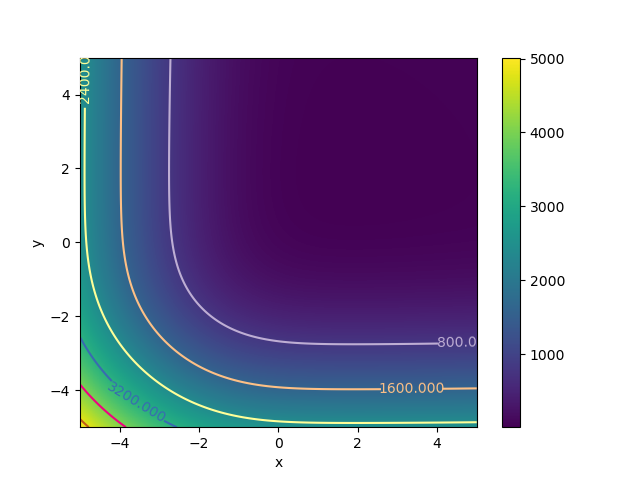
\includegraphics[scale=0.8]{handin/plt52}
%%     \caption{Classification of the test set}
%%   \end{subfigure}
%%   \caption{Exercise 5: Logistic Regression Applied to the Datasets}
%%   \label{plt5}
%% \end{figure}

\end{document}

